\let\negmedspace\undefined
\let\negthickspace\undefined
\documentclass[journal]{IEEEtran}
\usepackage[a5paper, margin=10mm, onecolumn]{geometry}
\usepackage{lmodern} % Ensure lmodern is loaded for pdflatex
\usepackage{tfrupee} % Include tfrupee package

\setlength{\headheight}{1cm} % Set the height of the header box
\setlength{\headsep}{0mm}  % Set the distance between the header box and the top of the text

\usepackage{csquotes}
\usepackage{gvv-book}
\usepackage{gvv}
\usepackage{circuitikz}
\usepackage{cite}
\usepackage{amsmath,amssymb,amsfonts,amsthm}
\usepackage{algorithmic}
\usepackage{graphicx}
\usepackage{textcomp}
\usepackage{xcolor}
\usepackage{txfonts}
\usepackage{listings}
\usepackage{enumitem}
\usepackage{mathtools}
\usepackage{gensymb}
\usepackage{comment}
\usepackage[breaklinks=true]{hyperref}
\usepackage{tkz-euclide} 
\usepackage{listings}
% \usepackage{gvv}                                        
\def\inputGnumericTable{}                                 
\usepackage[latin1]{inputenc}                                
\usepackage{color}                                            
\usepackage{array}                                            
\usepackage{longtable}                                       
\usepackage{calc}                                             
\usepackage{multirow}                                         
\usepackage{hhline}                                           
\usepackage{ifthen}                                           
\usepackage{lscape}
\usepackage{caption}
\usepackage{tikz}
\usetikzlibrary{patterns}
\begin{document}

\bibliographystyle{IEEEtran}



\title{GATE 2024 CIVIL ENGINEERING}
\author{EE25BTECH11013 - Bhargav}
\maketitle
% \maketitle
% \newpage
% \bigskip
{\let\newpage\relax\maketitle}

\renewcommand{\thefigure}{\theenumi}
\renewcommand{\thetable}{\theenumi}
\setlength{\intextsep}{10pt} % Space between text and floats


\section*{General Aptitude (GA)}
\section*{Q.1 -- Q.5 Carry ONE mark Each}
\begin{enumerate}

\item If '$\rightarrow$' denotes increasing order of intensity, then the meaning of the words  
[simmer $\rightarrow$ seethe $\rightarrow$ smolder] is analogous to  
[break $\rightarrow$ raze $\rightarrow$  $\_\_\_\_$].  
Which one of the given options is appropriate to fill the blank?  
\hfill \brak{GATE \ CE \ 2024} 
\begin{enumerate}
\item obfuscate
\item obliterate
\item fracture
\item fissure
\end{enumerate}

\item In a locality, the houses are numbered in the following way:  
The house-numbers on one side of a road are consecutive odd integers starting from $301$, while the house-numbers on the other side of the road are consecutive even numbers starting from $302$. The total number of houses is the same on both sides of the road.  
If the difference of the sum of the house-numbers between the two sides of the road is $27$, then the number of houses on each side of the road is  
\hfill \brak{GATE \ CE \ 2024}
\begin{enumerate}
\begin{multicols}{4}
\item $27$
\item $52$
\item $54$
\item $26$    
\end{multicols}
\end{enumerate}

\item For positive integers $p$ and $q$, with $\frac{p}{q} \neq 1$,  
$$\left(\frac{p}{q}\right)^{\frac{p}{q}} = p^{\left(\frac{p}{q} - 1\right)}.$$  
Then,  
\hfill \brak{GATE \ CE \ 2024}
\begin{enumerate}
\item $q^p = p^q$  
\item $q^p = p^{2q}$  
\item $\sqrt{q} = \sqrt{p}$  
\item $\sqrt[q]{q} = \sqrt[p]{p}$  
\end{enumerate}

\item Which one of the given options is a possible value of $x$ in the following sequence?  
$$3, \ 7, \ 15, \ x, \ 63, \ 127, \ 255$$  
\hfill \brak{GATE \ CE \ 2024}
\begin{enumerate}
\begin{multicols}{4}
\item $35$
\item $40$
\item $45$
\item $31$    
\end{multicols}
\end{enumerate}

\item On a given day, how many times will the second-hand and the minute -- hand of a clock cross each other during the clock time 12:05:00 hours to 12:55:00 hours?  
\hfill \brak{GATE \ CE \ 2024}
\begin{enumerate}
\begin{multicols}{4}
\item $51$
\item $49$
\item $50$
\item $55$
\end{multicols}
\end{enumerate}

\item In the given text, the blanks are numbered (i) -- (iv). Select the best match for all the blanks.  

From the ancient Athenian arena to the modern Olympic stadiums, athletics (i) $\_\_\_\_$ the potential for a spectacle. The crowd (ii) $\_\_\_\_$ with bated breath as the Olympian artist twists his body, stretching the javelin behind him. Twelve strides in, he begins to cross-step. Six cross-steps (iii) $\_\_\_\_$ in an abrupt stop on his left foot. As his body (iv) $\_\_\_\_$ like a door turning on a hinge, the javelin is launched skyward at a precise angle.  
\hfill \brak{GATE \ CE \ 2024}  
\begin{enumerate}
\item (i) hold, (ii) waits, (iii) culminates, (iv) pivot  
\item (i) holds, (ii) wait, (iii) culminates, (iv) pivot  
\item (i) hold, (ii) wait, (iii) culminate, (iv) pivots  
\item (i) holds, (ii) waits, (iii) culminate, (iv) pivots  
\end{enumerate}

\item Three distinct sets of indistinguishable twins are to be seated at a circular table that has $8$ identical chairs. Unique seating arrangements are defined by the relative positions of the people.  
How many unique seating arrangements are possible such that each person is sitting next to their twin?  
\hfill \brak{GATE \ CE \ 2024}  
\begin{enumerate}
\begin{multicols}{4}
\item $12$
\item $14$
\item $10$
\item $28$
\end{multicols}
\end{enumerate}

\item The chart given below compares the Installed Capacity (MW) of four power generation technologies, T1, T2, T3, and T4, and their Electricity Generation (MWh) in a time of $1000$ hours ($h$).  
\begin{figure}[H]
    \centering
    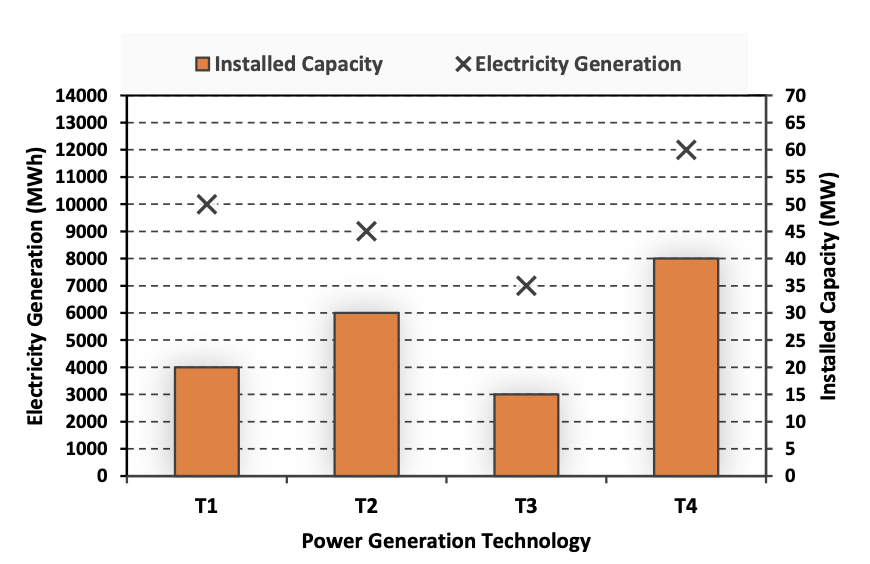
\includegraphics[width=0.6\columnwidth]{figs/Q8.png} 
    \caption{}
    \label{fig:placeholder}
\end{figure}
The Capacity Factor of a power generation technology is:  
$$\text{Capacity Factor} = \frac{\text{Electricity Generation (MWh)}}{\text{Installed Capacity (MW)} \times 1000 \ (h)}$$  
Which one of the given technologies has the highest Capacity Factor?  
\hfill \brak{GATE \ CE \ 2024}  
\begin{enumerate}
\begin{multicols}{4}
\item T1
\item T2
\item T3
\item T4    
\end{multicols}
\end{enumerate}

\item In the $4 \times 4$ array shown below, each cell of the first three columns has either a cross (X) or a number, as per the given rule.  

\begin{figure}[H]
    \centering
    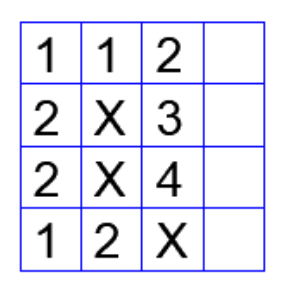
\includegraphics[width=0.3\columnwidth]{figs/Q9.png} 
    \caption{}
    \label{fig:placeholder}
\end{figure}

Rule: The number in a cell represents the count of crosses around its immediate neighboring cells (left, right, top, bottom, diagonals).  
As per this rule, the maximum number of crosses possible in the empty column is  
\hfill \brak{GATE \ CE \ 2024}  
\begin{enumerate}
\begin{multicols}{4}
\item $0$
\item $1$
\item $2$
\item $3$
\end{multicols}
\end{enumerate}

\item During a half-moon phase, the Earth-Moon-Sun form a right triangle. If the Moon-Earth-Sun angle at this half-moon phase is measured to be $89.85^\degree$, the ratio of the Earth-Sun and Earth-Moon distances is closest to  
\hfill \brak{GATE \ CE \ 2024}  
\begin{enumerate}
\begin{multicols}{4}
\item $328$
\item $382$
\item $238$
\item $283$   
\end{multicols}
\end{enumerate}

\section*{CE -- CIVIL ENGINEERING}

\section*{Q.11 -- Q.35 Carry ONE mark Each}

\item The smallest positive root of the equation  
$$x^5 - 5x^4 - 10x^3 + 50x^2 + 9x - 45 = 0$$  
lies in the range  
\hfill \brak{GATE \ CE \ 2024}  
\begin{enumerate}
\begin{multicols}{4}
\item $0 < x \leq 2$
\item $2 < x \leq 4$
\item $6 \leq x \leq 8$
\item $10 \leq x \leq 100$
\end{multicols}
\end{enumerate}

\item The second-order differential equation in an unknown function $u: u(x,y)$ is defined as  
$$\frac{\partial^2 u}{\partial x^2} = 2.$$  
Assuming $g: g(x)$, $f: f(y)$, and $h: h(y)$, the general solution of the above differential equation is  
\hfill \brak{GATE \ CE \ 2024}  
\begin{enumerate}
\item $u = x^2 + f(y) + g(x)$
\item $u = x^2 + x f(y) + h(y)$
\item $u = x^2 + x f(y) + g(x)$
\item $u = x^2 + f(y) + y g(x)$
\end{enumerate}

\item The probability that a student passes only in Mathematics is $\tfrac{1}{3}$.  
The probability that the student passes only in English is $\tfrac{4}{9}$.  
The probability that the student passes in both of these subjects is $\tfrac{1}{6}$.  
The probability that the student will pass in at least one of these two subjects is  
\hfill \brak{GATE \ CE \ 2024}  
\begin{enumerate}
\begin{multicols}{4}
\item $\tfrac{17}{18}$
\item $\tfrac{11}{18}$
\item $\tfrac{14}{18}$
\item $\tfrac{1}{18}$
\end{multicols}
\end{enumerate}

\item The three -- dimensional state of stress at a point is given by  
\begin{align}
\sigma = \myvec{$10$ & $0$ & $0$ \\ $0$ & $40$ & $0$ \\ $0$ & $0$ & $0$} \text{ MPa}. 
\end{align}
The maximum shear stress at the point is  
\hfill \brak{GATE \ CE \ 2024}  
\begin{enumerate}
\begin{multicols}{4}
\item $20$ MPa
\item $15$ MPa
\item $5$ MPa
\item $25$ MPa
\end{multicols}
\end{enumerate}

\item Concrete of characteristic strength $30$ MPa is required. If $40$ specimens of concrete cubes are to be tested, the minimum number of specimens having at least $30$ MPa strength should be  
\hfill \brak{GATE \ CE \ 2024}  
\begin{enumerate}
\begin{multicols}{4}
\item $35$
\item $37$
\item $38$
\item $39$
\end{multicols}
\end{enumerate}

\item Consider the statements P and Q.  \\
P: Client's Preliminary Estimate is used for budgeting costs toward the end of planning and design phase.  \\
Q: Client's Detailed Estimate is used for controlling costs during the execution of the project.  \\
Which one of the following options is CORRECT?  
\hfill \brak{GATE \ CE \ 2024}  
\begin{enumerate}
\item Both P and Q are TRUE
\item P is TRUE and Q is FALSE
\item Both P and Q are FALSE
\item P is FALSE and Q is TRUE
\end{enumerate}

\item The correct sequence of removing the Shores/Props for casting a cantilever RC beam is  
\hfill \brak{GATE \ CE \ 2024}  
\begin{figure}[H]
    \centering
    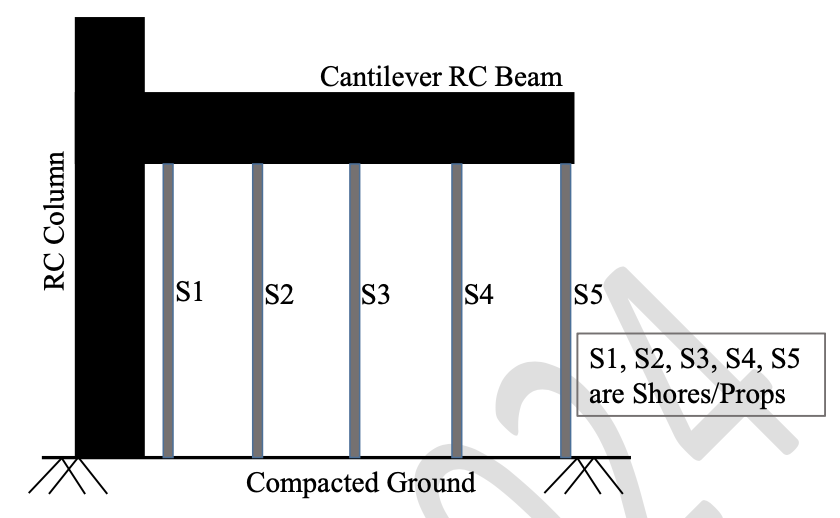
\includegraphics[width=0.6\columnwidth]{figs/Q17.png} 
    \caption{}
    \label{fig:placeholder}
\end{figure}
\begin{enumerate}
\item S1 $\rightarrow$ S2 $\rightarrow$ S3 $\rightarrow$ S4 $\rightarrow$ S5
\item S5 $\rightarrow$ S4 $\rightarrow$ S3 $\rightarrow$ S2 $\rightarrow$ S1
\item S3 $\rightarrow$ S2 $\rightarrow$ S4 $\rightarrow$ S1 $\rightarrow$ S5
\item S3 $\rightarrow$ S4 $\rightarrow$ S2 $\rightarrow$ S5 $\rightarrow$ S1
\end{enumerate}

\item A $2 \ m$ wide strip footing is founded at a depth of $1.5 \ m$ below the ground level in a homogeneous pure clay bed. The clay bed has unit cohesion of $40$ kPa. Due to seasonal fluctuations of water table from peak summer to peak monsoon period, the net ultimate bearing capacity of the footing, as per Terzaghi's theory, will  
\hfill \brak{GATE \ CE \ 2024}  
\begin{enumerate}
\begin{multicols}{4}
\item remain the same
\item decrease
\item increase
\item become zero
\end{multicols}
\end{enumerate}

\item Consider the statements P and Q.  \\
P: Soil particles formed by mechanical weathering, and close to their origin are generally subrounded.  \\
Q: Activity of the clay physically signifies its swell potential.  \\
Which one of the following options is CORRECT?  
\hfill \brak{GATE \ CE \ 2024}  
\begin{enumerate}
\item Both P and Q are TRUE
\item P is TRUE and Q is FALSE
\item Both P and Q are FALSE
\item P is FALSE and Q is TRUE
\end{enumerate}

\item The number of degrees of freedom for a natural open channel flow with a mobile bed is  
\hfill \brak{GATE \ CE \ 2024}  
\begin{enumerate}
\begin{multicols}{4}
\item $2$
\item $3$
\item $4$
\item $5$
\end{multicols}
\end{enumerate}

\item The following table gives various components of Municipal Solid Waste (MSW) 
and a list of treatment/separation techniques.  

\begin{tabular}[12pt]{ |c| c| c| c| }
\hline
$\beta$ & Airplane A & Airplane B & Airplane C \\
\hline
$\beta = -5\,\mathrm{deg}$ & $-0.030$ & $-0.025$ & $0.040$\\
\hline
$\beta = 0\,\mathrm{deg}$ & $0$ & $0$ & $0$ \\
\hline
$\beta = 5\,\mathrm{deg}$ & $0.030$ & $0.025$ & $-0.040$\\
\hline
\end{tabular}


The CORRECT match is  
\hfill \brak{GATE \ CE \ 2024}  

\begin{enumerate}
\item P-iii, Q-iv, R-i, S-ii  
\item P-iv, Q-iii, R-ii, S-i  
\item P-iii, Q-iv, R-ii, S-i  
\item P-iv, Q-iii, R-i, S-ii  
\end{enumerate}


\item A car is travelling at a speed of $60$ km/hr on a section of a National Highway having a downward gradient of $2\%$. The driver suddenly observes a stopped vehicle at $130 \ m$ ahead and applies brake. If the brake efficiency is $60\%$, coefficient of friction is $0.7$, driver's reaction time is $2.5 \ s$, and $g = 9.81 \ m/s^2$, the distance (in meters) required to bring the car to a safe stop lies in the range  
\hfill \brak{GATE \ CE \ 2024}  
\begin{enumerate}
\begin{multicols}{4}
\item $126$ to $130$
\item $41$ to $45$
\item $33$ to $37$
\item $75$ to $79$
\end{multicols}
\end{enumerate}

\item As per ICAO, the basic runway length is increased by $x \%$ for every $y$ \brak{m} raise in elevation from the Mean Sea Level \brak{MSL}. The values of $x$ and $y$, respectively, are  
\hfill \brak{GATE \ CE \ 2024}  
\begin{enumerate}
\begin{multicols}{4}
\item $7\%$, $300 \ m$
\item $5\%$, $200 \ m$
\item $4\%$, $500 \ m$
\item $10\%$, $1000 \ m$
\end{multicols}
\end{enumerate}

\item Which one of the following statements related to bitumen is FALSE?  
\hfill \brak{GATE \ CE \ 2024}  
\begin{enumerate}
\item Kinematic viscosity is a measure of resistance to the flow of molten bitumen under gravity.  
\item Softer grade bitumen possesses higher softening point than hard grade bitumen.  
\item Flash point of bitumen is the lowest temperature at which application of a test flame causes vapours of the bitumen to catch an instant fire under specified test conditions.  
\item Ductility test is carried out on bitumen to test its adhesive property and ability to stretch.  
\end{enumerate}

\item If the number of sides resulting in a closed traverse is increased from three to four, the sum of the interior angles increases by  
\hfill \brak{GATE \ CE \ 2024}  
\begin{enumerate}
\begin{multicols}{4}
\item $90^\degree$
\item $180^\degree$
\item $270^\degree$
\item $360^\degree$
\end{multicols}
\end{enumerate}

\item A surveyor observes a zenith angle of $93^\degree 00' 00''$ during a theodolite survey. The corresponding vertical angle is  
\hfill \brak{GATE \ CE \ 2024}  
\begin{enumerate}
\begin{multicols}{4}
\item $-03^\degree 00' 00''$
\item $+03^\degree 00' 00''$
\item $-87^\degree 00' 00''$
\item $+87^\degree 00' 00''$
\end{multicols}
\end{enumerate}

\item Among the following statements relating the fundamental lines of a transit theodolite, which one is CORRECT?  
\hfill \brak{GATE \ CE \ 2024}  
\begin{enumerate}
\item The line of collimation must be perpendicular to the horizontal axis at its intersection with the vertical axis.  
\item The axis of altitude level must be perpendicular to the line of collimation.  
\item The axis of plate level must lie in a plane parallel to the vertical axis.  
\item The Vernier of vertical circle must read zero when the line of collimation is vertical.  
\end{enumerate}

\item For the PDE  
\begin{align}
x \frac{\partial^2 f}{\partial x^2} + y \frac{\partial^2 f}{\partial y^2} = \frac{x^2+y^2}{2},
\end{align}
which of the following option(s) is/are CORRECT?  
\hfill \brak{GATE \ CE \ 2024}  
\begin{enumerate}
\item elliptic for $x > 0$ and $y > 0$  
\item parabolic for $x > 0$ and $y > 0$  
\item elliptic for $x = 0$ and $y > 0$  
\item hyperbolic for $x < 0$ and $y > 0$  
\end{enumerate}

\item The elements that DO NOT increase the strength of structural steel are  
\hfill \brak{GATE \ CE \ 2024}  
\begin{enumerate}
\begin{multicols}{4}
\item Carbon
\item Manganese
\item Sulphur
\item Chlorine
\end{multicols}
\end{enumerate}

\item Consider a balanced doubly -- reinforced concrete section. If the material and other sectional properties remain unchanged, for which of the following cases will the section become under -- reinforced?  
\hfill \brak{GATE \ CE \ 2024}  
\begin{enumerate}
\item Area of tension reinforcement is increased.  
\item Area of compression reinforcement is increased.  
\item Area of tension reinforcement is decreased.  
\item Area of compression reinforcement is decreased.  
\end{enumerate}



\item The primary air pollutant(s) is/are  
\hfill \brak{GATE \ CE \ 2024}  
\begin{enumerate}
\item Sulphur dioxide
\item Lead
\item Ozone
\item Sulphuric acid
\end{enumerate}

\item Consider the data of $f(x)$ given in the table.  
\begin{align}
\begin{table}[h!]
\small
\setlength{\tabcolsep}{4pt}
\renewcommand{\arraystretch}{0.9}
\centering
\begin{tabular}{|c|c|c|p{1.8cm}|p{2.5cm}|c|}
\hline
Q. No & Type & Section & Key & Marks \\
\hline
1  & MCQ & GA & C         & 1 \\
\hline
2  & MCQ & GA & A         & 1 \\
\hline
3  & MCQ & GA & A         & 1 \\
\hline
4  & MCQ & GA & A         & 1 \\
\hline
5  & MCQ & GA & D         & 1 \\
\hline
6  & MCQ & GA & D         & \textbf{2} \\
\hline
7  & MCQ & GA & B         & 2 \\
\hline
8  & MCQ & GA & C         & 2 \\
\hline
9  & MCQ & GA & B         & 2 \\
\hline
10 & MCQ & GA & C         & 2 \\
\hline
11 & MCQ & EY & D         & 1 \\
\hline
12 & MCQ & EY & D         & 1 \\
\hline
13 & MCQ & EY & A; D      & 1 \\
\hline
14 & MCQ & EY & B         & 1 \\
\hline
15 & NAT & EY & 7.99 : 8.10 & 1 \\
\hline
16 & MCQ & EY & B         & 1 \\
\hline
17 & MCQ & EY & C         & 1 \\
\hline
18 & MCQ & EY & D         & 1 \\
\hline
19 & NAT & EY & 9.9 : 10.1  & 1 \\
\hline
20 & MCQ & EY & C         & 1 \\
\hline
21 & MCQ & EY & B         & 1 \\
\hline
22 & MCQ & EY & A         & 1 \\
\hline
23 & MCQ & EY & D         & 1 \\
\hline
24 & MCQ & EY & B         & 1 \\
\hline
25 & MCQ & EY & A         & 1 \\
\hline
26 & MCQ & EY & C         & 2 \\
\hline
27 & MCQ & EY & D         & 2 \\
\hline
28 & MCQ & EY & C         & 2 \\
\hline
29 & MCQ & EY & D         & 2 \\
\hline
30 & MCQ & EY & B         & 2 \\
\hline
31 & MCQ & EY & A         & 2 \\
\hline
32 & MCQ & EY & C         & 2 \\
\hline
33 & MCQ & EY & A         & 2 \\
\hline
34 & MCQ & EY & B         & 2 \\
\hline
35 & MCQ & EY & A         & 2 \\
\hline
36 & MCQ & EY & A         & 2 \\
\hline
37 & MCQ & EY & C         & 2 \\
\hline
38 & MCQ & EY & A         & 2 \\
\hline
39 & NAT & EY & 0.17 : 0.19 & 2 \\
\hline
40 & MCQ & EY & A         & 2 \\
\hline
41 & MCQ & EY & B         & 2 \\
\hline
42 & MCQ & EY & B         & 2 \\
\hline
43 & MCQ & EY & A         & 2 \\
\hline
44 & MCQ & EY & D         & 2 \\
\hline
45 & MCQ & EY & B         & 2 \\
\hline
46 & MCQ & EY & A         & 2 \\
\hline
47 & NAT & EY & 0.175 : 0.20 & 2 \\
\hline
48 & MCQ & EY & A         & 2 \\
\hline
49 & NAT & EY & 0.49 : 0.51  & 2 \\
\hline
50 & MCQ & EY & B         & 2 \\
\hline
51 & MCQ & EY & A         & 2 \\
\hline
52 & MCQ & EY & C         & 2 \\
\hline
53 & NAT & EY & 1660 : 1700 & 2 \\
\hline
54 & NAT & EY & 0.45 : 0.55 & 2 \\
\hline
55 & MCQ & EY & A         & 2 \\
\hline
\end{tabular}
\caption{GATE 2016 EY Answer Key Summary}
\end{table} 
\end{align}
The value of $f(1.5)$ estimated using second-order Newton's interpolation formula 
is \_\_\_\_\_\_\_\_\_ \brak{rounded \ off \ to \ 2 \ decimal \ places}.  
\hfill \brak{GATE \ CE \ 2024}
  

\item The plane frame shown has fixed support at joint A, hinge support at joint F, and roller support at joint I. In the figure, A to I indicate joints of the frame.  
If the axial deformations are neglected, the degree of kinematic indeterminacy is $\_\_\_\_\_$ \brak{in \ integer}.  

\begin{figure}[H]
    \centering
    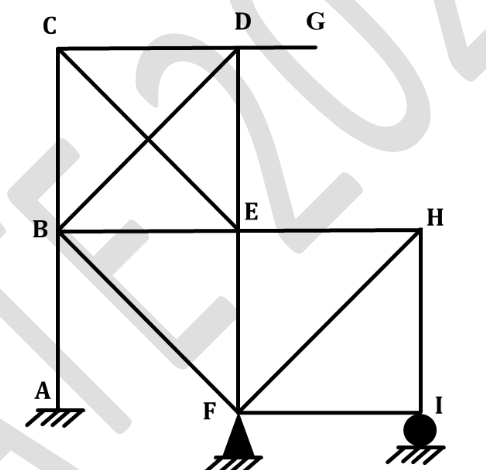
\includegraphics[width=0.3\columnwidth]{figs/Q33.png} 
    \caption{}
    \label{fig:placeholder}
\end{figure}
\hfill \brak{GATE \ CE \ 2024}  

\item An embankment is constructed with soil by maintaining the degree of saturation as $75\%$ during compaction. The specific gravity of soil is $2.68$ and the moisture content is $17\%$ during compaction. Consider $\gamma_w = 10 \ \text{kN/m}^3$.  
The dry unit weight (in kN/m$^3$) of the compacted soil is $\_\_\_\_\_$ \brak{rounded \ off \ to \ 2 \ decimal \ places}.  
\hfill \brak{GATE \ CE \ 2024}  

\item A $30 \ \text{cm}$ diameter well fully penetrates an unconfined aquifer of saturated thickness $20 \ \text{m}$ with hydraulic conductivity of $10 \ \text{m/day}$. Under the steady pumping rate for a long time, the drawdowns in two observation wells located at $10 \ \text{m}$ and $100 \ \text{m}$ from the pumping well are $5 \ \text{m}$ and $1 \ \text{m}$, respectively.  
The corresponding pumping rate (in m$^3$/day) from the well is $\_\_\_\_\_$ \brak{rounded \ off \ to \ 2 \ decimal \ places}.  
\hfill \brak{GATE \ CE \ 2024}  

\section*{Q.36 -- Q.65 Carry TWO marks Each}

\item What are the eigenvalues of the matrix  
\begin{align}
\myvec{$2$ & $1$ & $1$ \\ $1$ & $4$ & $1$ \\ $1$ & $1$ & $2$} ?
\end{align}

\hfill \brak{GATE \ CE \ 2024}  
\begin{enumerate}
\begin{multicols}{4}
\item $1,2,5$
\item $1,3,4$
\item $-5,1,2$
\item $-5,-1,2$
\end{multicols}
\end{enumerate}

\item A vector field $\vec{p}$ and a scalar field $r$ are given by  

\begin{align}
\vec{p} = (2x^2 - 3xy + z^2)\hat{i} + (2y^2 - 3yz + x^2)\hat{j} + (2z^2 - 3xz + x^2)\hat{k}, 
\end{align}

 
\begin{align}
r = 6x^2 + 4y^2 - z^2 - 9xyz - 2xy + 3xz - yz.
\end{align}
Consider the statements P and Q.  
P: Curl of the gradient of the scalar field $r$ is a null vector.  
Q: Divergence of curl of the vector field $\vec{p}$ is zero.  
Which one of the following options is CORRECT?  
\hfill \brak{GATE \ CE \ 2024}  
\begin{enumerate}
\item Both P and Q are FALSE
\item P is TRUE and Q is FALSE
\item P is FALSE and Q is TRUE
\item Both P and Q are TRUE
\end{enumerate}

\item Find the correct match between the plane stress states and the Mohr's circles.

\begin{figure}[H]
    \centering
    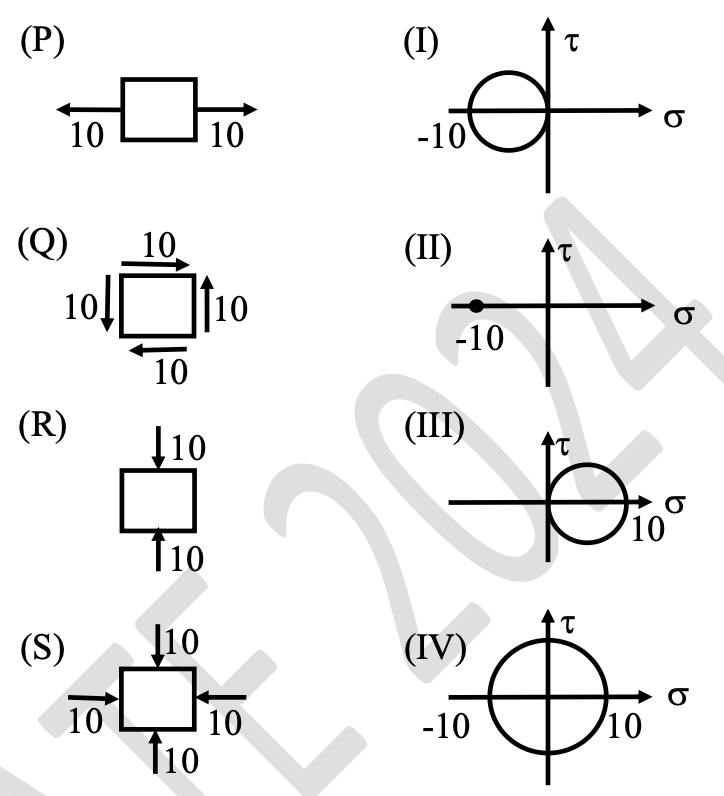
\includegraphics[width=0.3\columnwidth]{figs/Q38.png} 
    \caption{}
    \label{fig:placeholder}
\end{figure}
\hfill \brak{GATE \ CE \ 2024}  
\begin{enumerate}
\item (P)-(III); (Q)-(IV); (R)-(I); (S)-(II)  
\item (P)-(III); (Q)-(II); (R)-(I); (S)-(IV)  
\item (P)-(I); (Q)-(IV); (R)-(III); (S)-(II)  
\item (P)-(I); (Q)-(II); (R)-(III); (S)-(IV)  
\end{enumerate}

\item The beam shown is subjected to a uniformly distributed downward load of intensity $q$ between supports A and B. Considering the upward reactions as positive, the support reactions are  
\begin{figure}[H]
    \centering
    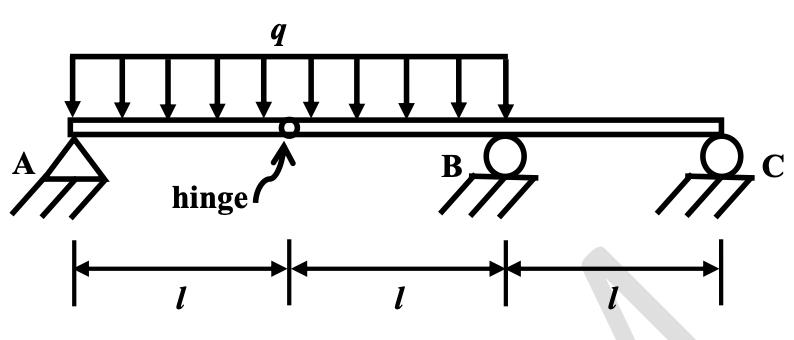
\includegraphics[width=0.6\columnwidth]{figs/Q39.png} 
    \caption{}
    \label{fig:placeholder}
\end{figure}
\hfill \brak{GATE \ CE \ 2024}  
\begin{enumerate}
\item $R_A = \frac{ql}{2}, \ R_B = \frac{5ql}{2}, \ R_C = -ql$  
\item $R_A = -ql, \ R_B = \frac{5ql}{2}, \ R_C = \frac{ql}{2}$  
\item $R_A = -\frac{ql}{2}, \ R_B = \frac{5ql}{2}, \ R_C = 0$  
\item $R_A = \frac{ql}{2}, \ R_B = ql, \ R_C = \frac{ql}{2}$  
\end{enumerate}

\item A homogeneous shaft PQR with fixed supports at both ends is subjected to a torsional moment $T$ at point Q. The polar moments of inertia of the portions PQ and QR are $J_1$ and $J_2$. The torsional moment reactions at the supports are $T_P$ and $T_R$.  
If $\tfrac{T_P}{T_R} = 4$ and $\tfrac{J_1}{J_2} = 2$, the ratio $\tfrac{L_1}{L_2}$ is  
\hfill \brak{GATE \ CE \ 2024}  

\begin{figure}[H]
    \centering
    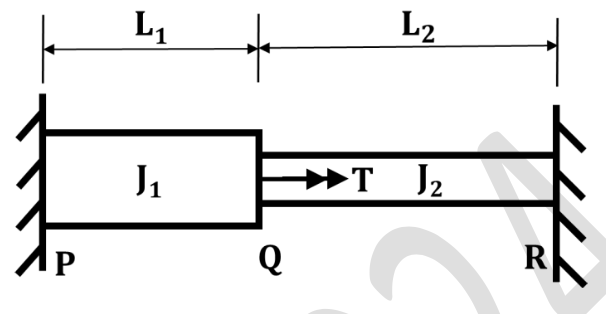
\includegraphics[width=0.6\columnwidth]{figs/Q40.png} 
    \caption{}
    \label{fig:placeholder}
\end{figure}

\begin{enumerate}
\begin{multicols}{4}
\item $0.50$
\item $0.25$
\item $4.00$
\item $2.00$
\end{multicols}
\end{enumerate}

\item A vertical smooth rigid retaining wall is supporting horizontal ground with dry cohesionless backfill having a friction angle of $30^\degree$. The inclinations of failure planes with respect to the major principal plane for Rankine's active and passive earth pressure conditions, respectively, are  
\hfill \brak{GATE \ CE \ 2024}  
\begin{enumerate}
\begin{multicols}{4}
\item $30^\degree, 30^\degree$
\item $60^\degree, 60^\degree$
\item $30^\degree, 60^\degree$
\item $60^\degree, 30^\degree$
\end{multicols}
\end{enumerate}

\item A flow velocity field $\vec{V}(x,y)$ for a fluid is represented by  
\begin{align}
\vec{V} = 3\hat{i} + (5x)\hat{j}.
\end{align}
Which one of the following statements is CORRECT?  
\hfill \brak{GATE \ CE \ 2024}  
\begin{enumerate}
\item The fluid is incompressible and the flow is rotational.  
\item The fluid is incompressible and the flow is irrotational.  
\item The fluid is compressible and the flow is rotational.  
\item The fluid is compressible and the flow is irrotational.  
\end{enumerate}

\item For assessing compliance with emission standards of incineration plants: HCl limit = 50 mg/Nm$^3$ (at 11\% O$_2$). Measured: HCl = 42 mg/Nm$^3$, O$_2$ = 13\%. Assuming 21\% O$_2$ in air, the correct statement is  
\hfill \brak{GATE \ CE \ 2024}  
\begin{enumerate}
\item No compliance, as the corrected HCl emission is greater than the emission standard.  
\item Compliance is there, as the corrected HCl emission is lesser than the emission standard.  
\item Compliance is there, as there is no need to apply the correction since O$_2 > 11\%$ and HCl emission is lesser than the standard.  
\item No compliance, as O$_2 > 11\%$ in the flue gas.  
\end{enumerate}

\item The free mean speed is $60$ km/hr on a given road. The average space headway at jam density is $8 \ m$. For a linear speed-density relationship, the maximum flow (veh/hr/lane) is  
\hfill \brak{GATE \ CE \ 2024}  
\begin{enumerate}
\begin{multicols}{4}
\item $1875$
\item $938$
\item $2075$
\item $1038$
\end{multicols}
\end{enumerate}

\item A map is prepared with a scale of $1:1000$ and a contour interval of $1 \ m$. If the distance between two adjacent contours on the map is $10 \ mm$, the slope of the ground between the adjacent contours is  
\hfill \brak{GATE \ CE \ 2024}  
\begin{enumerate}
\begin{multicols}{4}
\item $30\%$
\item $10\%$
\item $35\%$
\item $40\%$
\end{multicols}
\end{enumerate}

\item Which of the following statement(s) is/are CORRECT?  
\hfill \brak{GATE \ CE \ 2024}  
\begin{enumerate}
\item Swell potential of soil decreases with an increase in the shrinkage limit.  
\item Both loose and dense sands with different initial void ratios can attain similar void ratio at large strain during shearing.  
\item Among the several corrections to be applied to the SPT-N value, the dilatancy correction is applied before all other corrections.  
\item In electrical resistivity tomography, the depth of current penetration is half of the spacing between the electrodes.  
\end{enumerate}

\item The return period of a large earthquake for a given region is 200 years. Assuming Poisson distribution, the probability that it will be exceeded at least once in 50 years is $\_\_\_\_\_$ \% (rounded off to nearest integer).  
\hfill \brak{GATE \ CE \ 2024}  

\item A $2 \times 2 \ m$ tank of $3 \ m$ height has inflow, outflow and stirring. Initially half-filled. At $t=0$, inflow = $2$ L/s of $5 \ g/m^3$ salt solution, outflow = $1$ L/s well-mixed. Model:  
\begin{align}
\frac{dm}{dt} + \frac{m}{6000+t} = 0.01
\end{align}
where $m$ is the salt mass in grams. The mass of salt in the tank at 75\% capacity is $\_\_\_\_\_$ g \brak{rounded \ off \ to \ 2 \ decimal \ places}.  
\hfill \brak{GATE \ CE \ 2024}  

\item A plane truss with $13$ joints and $22$ members, supports at A (pin), L (pin) and K (roller). Loads: $10$ kN downward at H and $10$ kN horizontal at B. The magnitude of the reaction \brak{in \ kN} at support L is $\_\_\_\_\_$ (rounded off to 1 decimal place).  
\hfill \brak{GATE \ CE \ 2024}  
\begin{figure}[H]
    \centering
    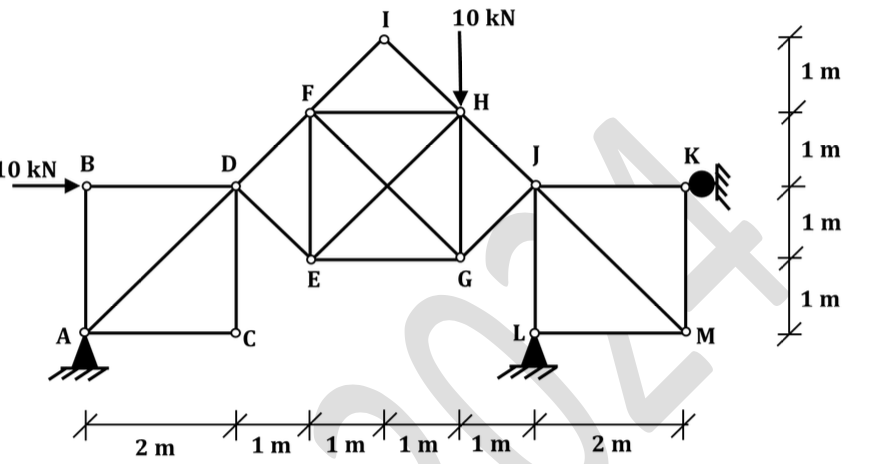
\includegraphics[width=0.6\columnwidth]{figs/Q49.png} 
    \caption{}
    \label{fig:placeholder}
\end{figure}


\item An inverted T -- shaped beam B1 is prestressed with 1000 kN force at kern point. Beam B2 is identical without prestress. The additional cracking moment (kN·m) carried by B1 in comparison to B2 is $\_\_\_\_\_$ \brak{rounded \ off \ to \ nearest \ integer}.  
\hfill \brak{GATE \ CE \ 2024}  

\begin{figure}[H]
    \centering
    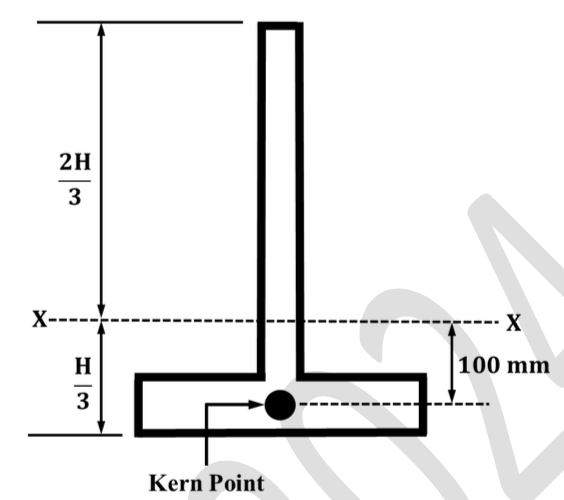
\includegraphics[width=0.6\columnwidth]{figs/Q50.png} 
    \caption{}
    \label{fig:placeholder}
\end{figure}

\item Equipment cost = Rs. $1,00,000$. Salvage value = Rs. $10,000$ at $5$ years. Find the difference in depreciation (Rs.) between double-declining balance and straight-line methods in Year -- 2.  
\hfill \brak{GATE \ CE \ 2024}  

\item A slab panel with an effective depth of $250$ mm is reinforced with 0.2 percent main
reinforcement using $8$ mm diameter steel bars. The uniform center -- to -- center
spacing \brak{in / mm} at which the $8$ mm diameter bars are placed in the slab panel is $\_\_\_\_\_$ \brak{rounded \ off \ to \ nearest \ integer}.  
\hfill \brak{GATE \ CE \ 2024}  

\item The total primary consolidation settlement \brak{S_c} of a building constructed on a $10$ m thick saturated clay layer is estimated to be $50$ mm. After $300$ days of the
construction of the building, primary consolidation settlement was reported as
10 mm. The additional time \brak{in \ days} required to achieve $50$ percent of \brak{S_c} will be$\_\_\_\_\_$ \brak{rounded \ off}.  
\hfill \brak{GATE \ CE \ 2024}  

\item An infinite slope is made up of cohesionless soil with seepage parallel to and up to
the sloping surface. The angle of slope is $30$\degree with respect to horizontal ground
surface. The unit weights of the saturated soil and water are $20$ kN/m$^3$ and $10$ kN/m$^3$,  respectively. The minimum angle of shearing resistance of the soil \brak{in \ degrees} for the critically stable condition of the slope is  
\hfill \brak{GATE \ CE \ 2024}  

\item A soil sample was consolidated at a cell pressure of 20 kPa and a back pressure of
10 kPa for 24 hours during a consolidated undrained (CU) triaxial test. The cell
pressure was increased to 30 kPa on the next day and it resulted in the development
of pore water pressure of 1 kPa. The soil sample failed when the axial stress was
gradually increased to 50 kPa. The pore water pressure at failure was recorded as
21 kPa. The value of Skempton's pore pressure parameter B for the soil sample is $\_\_\_\_\_$ \brak{rounded \ off \ to \ 2 \ decimal \ places}.  
\hfill \brak{GATE \ CE \ 2024}  

\item The ordinates of a 1-hour unit hydrograph (UH) are given below. \hfill \brak{GATE \ CE \ 2024}

\begin{center}
\begin{tabular}{|p{1cm}|p{3cm}|p{1cm}|p{7cm}|}
\hline

\multicolumn{2}{|c|}{Process} & \multicolumn{2}{c|}{Application} \\
\hline
P & Extrusion & 1 & Producing complex parts with close tolerance \\
\hline
Q & Injection molding & 2 & Producing thermosetting plastic components \\
\hline
R & Blow molding & 3 & Producing long uniform sections \\
\hline
S & Compression molding & 4 & Producing hollow shapes \\
\hline
\end{tabular}
\end{center} 
\begin{tabular}[12pt]{ |c| c| c| c| c| c| }
    \hline
   Q.No. & Session & Que.Type & Sec. Name & Key & Marks \\
    \hline
    46 & 4 & NAT & AE & 149.0 to 151.0 & 2\\
    \hline
    47 & 4 & NAT & AE & 1712.0 to 1719.0 & 2\\
    \hline
    48 & 4 & NAT & AE & 91 to 93 & 2\\
    \hline
    49 & 4 & NAT & AE & 87 to 89 & 2\\
    \hline
    50 & 4 & NAT & AE & 27.0 to 27.2 & 2\\
    \hline
    51 & 4 & NAT & AE & 1.43 to 1.45 & 2\\
    \hline
    52 & 4 & NAT & AE & 0.61 to 0.63 & 2\\
    \hline
    53 & 4 & NAT & AE & 3.74 to 3.76 & 2\\
    \hline
    54 & 4 & NAT & AE & 62.95 to 63.08 & 2\\
    \hline
    55 & 4 & NAT & AE & 57.10 to 60.00 & 2\\
    \hline
\end{tabular}



These ordinates are used to derive a 3-hour UH. The peak discharge (in m$^3$/s) for the derived 3-hour UH is \underline{\hspace{2cm}} (rounded off to the nearest integer).

\hfill \brak{GATE \ CE \ 2024}  

\item A standard round bottom triangular canal has bed slope 1 in 200,  Chezy's coefficient = $150$. For $Q=20$ m$^3$/s, the normal depth $y$ \brak{m} is $\_\_\_\_\_$ (rounded off to 2 decimal places).  
\hfill \brak{GATE \ CE \ 2024}  

\begin{figure}[H]
    \centering
    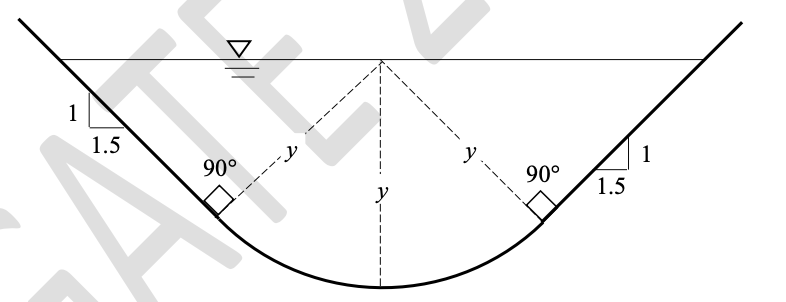
\includegraphics[width=0.6\columnwidth]{figs/Q57.png} 
    \caption{}
    \label{fig:placeholder}
\end{figure}

\item A spillway has unit discharge $7.5$ m$^3$/s/m. Flow depth downstream = $0.5$ m. The tail water depth \brak{m} required to form a hydraulic jump is $\_\_\_\_\_$ \brak{rounded \ off \ to \ 2 \ decimal \ places}.  
\hfill \brak{GATE \ CE \ 2024}  

\item A 5 m $\times$ $5$ m tank of $10$ m height contains water and oil, connected to an overhead reservoir. $\gamma_w = 10$ kN/m$^3$, specific gravity of oil = $0.8$. The total force \brak{kN} due to pressure on side PQR is $\_\_\_\_\_$ \brak{rounded \ off \ to \ nearest \ integer}.  
\hfill \brak{GATE \ CE \ 2024}  
\begin{figure}[H]
    \centering
    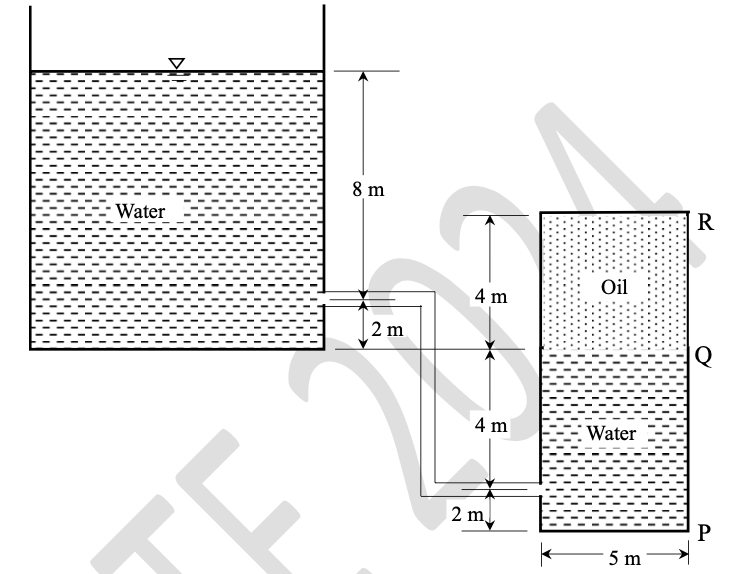
\includegraphics[width=0.6\columnwidth]{figs/Q59.png} 
    \caption{}
    \label{fig:placeholder}
\end{figure}


\item Activated carbon removes pollutant in a batch reactor (first-order, $k=0.38$/day). Time (days) required to remove 95\% pollutant is $\_\_\_\_\_$ \brak{rounded \ off \ to \ 1 \ decimal \ place}.  
\hfill \brak{GATE \ CE \ 2024}  

\item A water treatment plant treats $25$ MLD water with alkalinity 4.0 mg/L (as CaCO$_3$). During coagulation, $450$ kg/day Ca(HCO$_3$)$_2$ is required. Find pure CaO required (kg/day).  
\hfill \brak{GATE \ CE \ 2024}  

\item The number of trains and their corresponding speeds for a curved Broad Gauge 
section with 437 m radius, are 

\begin{itemize}
\item 20 trains travel at a speed of 40 km/hr 
\item 15 trains travel at a speed of 50 km/hr 
\item 12 trains travel at a speed of 60 km/hr 
\item 8 trains travel at a speed of 70 km/hr 
\item 3 trains travel at a speed of 80 km/hr 
\end{itemize}
If the gauge (center -- to -- center distance between the rail heads) is taken as 1750 mm, 
the required equilibrium cant \brak{in mm} will be \_\_\_\_\_\_\_\_\_\_\_\_\_ \brak{rounded \ off \ to \ the \  nearest \ integer}.  
\hfill \brak{GATE \ CE \ 2024}


\item Six vehicle trajectories in a time -- space domain are shown. The mean speed (km/hr) of vehicles is $\_\_\_\_\_$ \brak{rounded \ off \ to \ nearest \ integer}.  
\hfill \brak{GATE \ CE \ 2024}  

\begin{figure}[H][H]
    \centering
    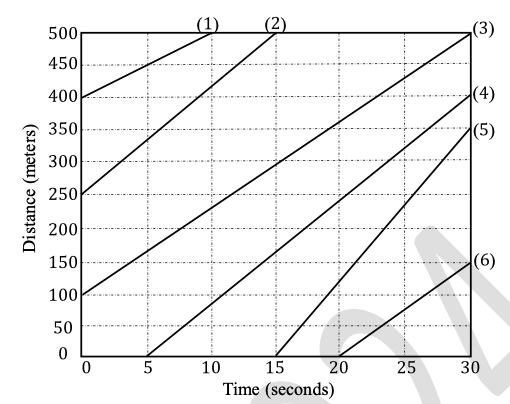
\includegraphics[width=0.6\columnwidth]{figs/Q63.png} 
    \caption{}
    \label{fig:placeholder}
\end{figure}

\item Axle load survey: average rear axle load = $12000$ kg, $800$ CV/day. Pavement reconstructed after $5$ years, design life $15$ years. Annual growth = $4\%$. Standard axle load = 8160 kg. Cumulative standard axle \brak{msa} = $\_\_\_\_\_$ \brak{rounded \ off \ to\  2 \ decimal \ places}.  
\hfill \brak{GATE \ CE \ 2024}  

\item A bird is at point P at height 8 m above MSL. Flies to point Q at 3 m above MSL. Ground slope = 1 in 2. Ignoring curvature and refraction, horizontal distance (m) between P and Q is $\_\_\_\_\_$ \brak{in \ integer}.  
\hfill \brak{GATE \ CE \ 2024}  









\end{enumerate}




\end{document}
